\documentclass{article}
\usepackage[a4paper, margin={1in, 1in}]{geometry}
\usepackage[utf8]{inputenc}
\usepackage{polski}
\usepackage{mathtools}
\usepackage{amsfonts}
\usepackage{amssymb}
\usepackage{amsmath}
\usepackage{multicol}
\usepackage{paralist}
\usepackage{tabto}
\usepackage{graphicx}
\usepackage{etoolbox}
\usepackage{changepage}
\usepackage{tasks}
\usepackage{pgfplots}
\usepackage{fancyhdr}

\DeclareMathOperator{\arctg}{arctg}
\DeclareMathOperator{\tg}{tg}
\DeclareMathOperator{\sh}{sh}
\DeclareMathOperator{\ch}{ch}
\DeclareMathOperator{\sgn}{sgn}

\let\arctan\relax
\DeclareMathOperator{\arctan}{arctg}
\let\tan\relax
\DeclareMathOperator{\tan}{tg}

% Dodatkowe deklaracje:

% Koniec dodatkowych deklaracji

\pagestyle{fancy}

\lhead{Metody numeryczne, zestaw 2; 2020/2021}
% Tutaj proszę uzupełnić imię i nazwisko
\rhead{Wojciech Szlosek}

\begin{document}

\section*{Zadanie 4}
Rozważmy wzór na sieczną: $W(x) = ax + b$. Oraz niech $W(x_k) = f(x_k)$. Mamy:
$$f(x_k) = ax_k + b \ \ \wedge \ \ f(x_{k-1}) = ax_{k-1}+b$$
$$f(x_k) - f(x_{k-1}) = a(x_k - x_{k-1})$$
$$a = \frac{f(x_k) - f(x_{k-1})}{x_k - x_{k-1}}$$
$$b = f(x_k) - ax_k = f(x_k) = f(x_k) - \frac{(f(x_k) - f(x_{k-1})) \cdot x_k}{x_k - x_{k-1}}$$ \\
$x_{k+1}$ to miejsce przecięcia siecznej z osią OX. \\
Mamy więc $f(x_{k+1}) = ax_{k+1}+b = 0 \ \implies \ x_{k+1} = \frac{-b}{a} = (-f(x_k) + \frac{(f(x_k) - f(x_{k-1})) \cdot x_k}{x_k - x_{k-1}}) \cdot \frac{x_k - x_{k-1}}{f(x_k) - f(x_{k-1})} = ... \\$
$$x_{k+1} = ... = x_k - \frac{f(x_k)(x_k - x_{k-1})}{f(x_k)-f(x_{k-1})} \ \ \ \ \ CND.$$ \\
Zauważmy, że obliczając $x_{k+1}$ potrzebujemy dwóch poprzednich składników (jako następstwo rekurencji). Może być zatem mowa o dwóch potrzebnych krokach tej metody (metody siecznych). \\ \\ \\
c) Rozważamy funkcję $f(x) = xe^{-x^2}$. Jej jedynym miejscem zerowym jest $x = 0$. Dla dowolnego argumentu $x > 0$, $f(x) > 0$. Wyznaczmy drugą pochodną:
$$f^{'}(x) = e^{-x^2} - 2e^{-x^2}x^2$$
$$f^{''}(x) = 4x^3 \cdot e^{-x^2} - 6x \cdot e^{-x^2} = (4x^3 - 6x) \cdot e^{-x^2}$$
Zauważmy, że funkcja będzie wypukła, wtedy, gdy druga pochodna będzie dodania.
$$(4x^3 - 6x) \cdot e^{-x^2} > 0$$
$$4x^3 - 6x > 0 \ \ \ \ \ x(4x^2 - 6) > 0$$
Z całą pewnością dodatnie np. dla $x > 3$. \\
Ustabilizujmy wnioski: dla $x > 3$, $f(x) > 0$ i $f^{''}(x) > 0$, a więc dla takich punktów startowych $x_1, x_2 > 3$ metoda siecznych będzie rozbieżna (ponieważ dla funkcji wypukłej i dodatniej, robiąc sieczną, przetnie ona oś OX daleko od 0, a w 0 jest miejsce zerowe). \\ \\
Odp.: Czyli np. dla punktów startowych $x_1 = 5, x_2 = 8$. \\ \\ \\
d) Można. Rozważmy poniższy rysunek (na następnej stronie). Analogicznie do podpunktu c), będziemy "oddalać się" od miejsca zerowego z każdym kolejnym punktem $x_n$. Metoda więc nie będzie wtedy zbieżna.

\begin{figure}[H]
\centering
  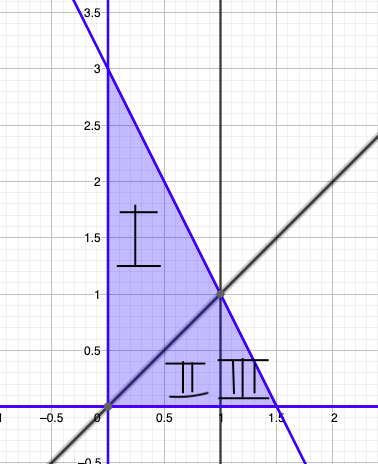
\includegraphics[scale=0.50]{k.png}
\end{figure}

\end{document}
